\documentclass[]{standalone}

\usepackage{pgf, tikz}
\usetikzlibrary{arrows, automata}
\usepackage{calc}

\begin{document}

    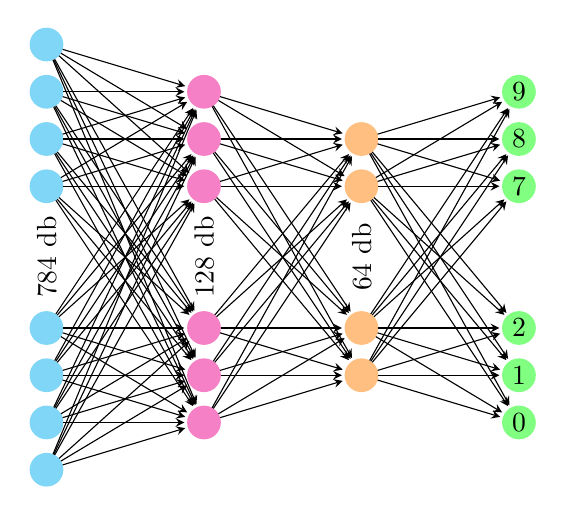
\begin{tikzpicture}[
            > = stealth, % arrow head style
            shorten > = 1pt, % don't touch arrow head to node
            auto,
            node distance = 0.8cm, % distance between nodes
%            semithick % line style
        ]

        \tikzstyle{every state}=[
            draw = cyan!50,
            thick,
            fill = cyan!50,
            minimum size = 4mm
        ]

        \node[state] (i1) at (0,0.6) {};
        \foreach \x in {2,3,4,7,8,9,10}
            \node[state] (i\x) at (0,\x*0.6) {};
            
        \node[rotate=90] at (0,5.5*0.6) {784 db};
        
        \tikzstyle{every state}=[
	        draw = magenta!50,
	        thick,
	        fill = magenta!50,
	        minimum size = 4mm
        ]
        
        \node[state] (j2) at (2,2*0.6) {};
        \foreach \x in {3,4,7,8,9}
        	\node[state] (j\x) at (2,\x*0.6) {};
        
        \node[rotate=90] at (2,5.5*0.6) {128 db};
        
        \tikzstyle{every state}=[
	        draw = orange!50,
	        thick,
	        fill = orange!50,
	        minimum size = 4mm
        ]
        
        \node[state] (k3) at (4,3*0.6) {};
        \foreach \x in {4,7,8}
        	\node[state] (k\x) at (4,\x*0.6) {};
        
        \node[rotate=90] at (4,5.5*0.6) {64 db};
        
        \tikzstyle{every state}=[
	        draw = green!50,
	        thick,
	        fill = green!50,
	        minimum size = 4mm,
	        inner sep=0cm
        ]
        
        \node[state] (l2) at (6,2*0.6) {0};
        \node[state] (l3) at (6,3*0.6) {1};
        \node[state] (l4) at (6,4*0.6) {2};
        \node[state] (l7) at (6,7*0.6) {7};
        \node[state] (l8) at (6,8*0.6) {8};
        \node[state] (l9) at (6,9*0.6) {9};
		
		\foreach \x in {1,2,3,4,7,8,9,10}
			\foreach \y in {2,3,4,7,8,9}
				\path[->] (i\x) edge (j\y);
				
		\foreach \y in {2,3,4,7,8,9}
			\foreach \x in {3,4,7,8}
				\path[->] (j\y) edge (k\x);
				

		\foreach \x in {3,4,7,8}
			\foreach \y in {2,3,4,7,8,9}
				\path[->] (k\x) edge (l\y);
		
%        \path[->] (s) edge node {18} (v1);
        %\path[->] (s) edge node {1} (v2);
        %\path[->] (s) edge node {1} (v3);
        %\path[->] (v2) edge node {2} (v1);
        %\path[->] (v3) edge node {1} (v2);
        %\path[->] (v1) edge node {20} (t);

        %\draw[red, dashed] (1, 2) -- (1, -2);
    \end{tikzpicture}

\end{document}
